\documentclass[]{beamer}

% Uključi hrvatski jezik
\RequirePackage[utf8]{inputenc}
\RequirePackage[croatian]{babel}

%\colorlet{structure}{green!50!black}

\beamertemplateshadingbackground{red!10}{blue!10}

\RequirePackage{graphicx}
\RequirePackage{booktabs}
\RequirePackage{multirow}
\usepackage{beamerthemeshadow}
\usepackage{amsmath,amssymb}
\usepackage{colortbl}


\beamertemplatetransparentcovereddynamic

\title[Raspoznavanje rukom pisanih slova]{Raspoznavanje rukom pisanih slova na ispitnim
obrascima} \author[T.~Grbin, M.~Komar, I.~Kravarščan, T.~Pivčević, I.~Stokić]{
Tomislav Grbin\\
Mihej Komar\\
Ivan Kravarščan\\
Toni Pivčević\\
Ivana Stokić
}

\institute[Sveučilište u Zagrebu]{
  Fakultet elektrotehnike i računarstva\\
  Sveučilište u Zagrebu}
\date[rujan 2008.]{Praktični rad iz predmeta Neuronske mreže}
\subject{SPUS}

\begin{document}

\titlepage

\frame
{
  \frametitle{Sadržaj}
  \tableofcontents
}

\section[Uvod]{Uvod}

\frame{
  \frametitle{Uvod}

  \begin{itemize}
  \item TODO
  \end{itemize}
}

\section[Koraci klasifikacije]{Koraci klasifikacije}

\subsection[Pretprocesiranje]{Pretprocesiranje slike}

\frame{
  \begin{itemize}
  \item Binariziranje slike
	\begin{itemize}
	\item Pronalazi se intenzitet takav da je bar pola slika svijetlije od njega
	\item Sve iznad toga se postavlja u bijelo, a sve ispod u crno
	\end{itemize}
  \item Uklanjanje rubova
    \begin{itemize}
	\item Rubovi različiti na svim uzorcima, eksperimentiranje s raznim idejama
	\item Uzima se u obzir širina ruba, profil boje ruba
	\item Problemi kad slovo dolazi do ruba
	\end{itemize}
  \end{itemize} 
}

\frame{
  \begin{itemize}
  \item Uklanjanje šuma
	  \begin{itemize}
	  \item U jednom prolazu se rubovi slova zagladuju, znatno smanjuju manje
	  skupine crnih piksela na bijeloj podlozi i obrnuto
	  \item U rijetkim slučajevima artefakti, ali ne utječu na rezultat
	  \end{itemize}
  \item Uklanjanje mrlja
	  \begin{itemize}
	  \item Veće i udaljenije skupine se uklanjaju sa slike
	  \item Uklanja točke, crte i mrlje udaljene od slova
	  \end{itemize}
  \end{itemize} 
}

\frame{
  \begin{itemize}
  \item Zumiranje slova
  \item Stanjivanje linija
	  \begin{itemize}
	  \item Iterativno uklanjanje crnih piksela
	  \item Normalizacija debljine linija na jedan piksel
	  \end{itemize}
  \end{itemize} 
}

\subsection[Izlučivanje značajki]{Izlučivanje značajki}

\frame{
  \begin{itemize}
  \item Gustoća po dijelovima slike
    \begin{itemize}
    \item Dijelimo sliku na 20x20 jednakih dijelova
	\item Gledamo odnos crnih i bijelih piksela unutar svakog dijela
    \end{itemize} 
  \item Broj presjecišta
    \begin{itemize}
    \item Broj presjecišta vodoravnih i okomitih linija sa slovom
    \end{itemize} 
  \item Profil slova
    \begin{itemize}
    \item Nađemo najmanji pravokutnik koji omeđuje slovo
	\item Za svaku točku pravokutnika računamo najmanju udaljenost do slova
	\item Na taj način opisujemo vanjski oblik slova
    \end{itemize} 
  \end{itemize} 
}

\frame{
  \begin{itemize}
  \item Histogram polovica slike
    \begin{itemize}
    \item Podijelimo sliku na gornji i donji dio
	\item Za svaki dio promatramo broj crnih piksela u svakom stupcu
	\item Slično radimo i za lijevu i desnu polovicu
    \end{itemize} 
  \item Radijalni histogram
    \begin{itemize}
    \item Tražimo broj crnih piksela na polupravcima koji kreću iz središta slova
    \end{itemize} 
  \item Hu-ovi invarijantni momenti
    \begin{itemize}
	\item Brojevi koji ne ovise o rotaciji, translaciji i veličini objekta
    \item Nije se pokazalo dovoljno dobrim
    \end{itemize} 
  \end{itemize} 
}

\subsection[Klasifikatori]{Klasifikatori}

\frame{
  \begin{itemize}
  \item Prepoznavanje praznih polja
  \end{itemize} 
}

\frame{
  \begin{itemize}
  \item Višeslojni perceptron
  \end{itemize} 
}

\frame{
  \begin{itemize}
  \item Radijalne neuronske mreže
    \begin{itemize}
    \item Nisu se pokazale dobrim
    \end{itemize} 
  \item Zajednica klasifikatora
  \end{itemize} 
}

\section[Rezultati]{Rezultati}

\subsection[Po klasifikatorima]{Po klasifikatorima}

\frame{
	\frametitle{Rezultati po klasifikatorima (1/2)}
	\begin{table}[htb]
	\centering
	\begin{tabular}{llr} \toprule
	Klasifikator & Značajke & Točnost \\
	\midrule
	\multirow{5}{3.5cm}{Višeslojni perceptron}
	 & Presjecišta & 86,70\% \\
	 & Gustoća & 88,34\% \\
	 & Histogram & 84,88\% \\
	 & Profili & 88,89\% \\
	 & Radijalni histogram & 88,52\% \\
	\midrule
	\multirow{3}{3.5cm}{K-najbližih susjeda}
	 & Histogram & 88,16\% \\
	 & Gustoća & 90,89\% \\
	 & Profili & 88,53\% \\
	\midrule
	\end{tabular}
	\center{\ldots}
	\end{table}
}

\frame{
\frametitle{Rezultati po klasifikatorima (2/2)}
	\center{\ldots}
	\begin{table}[htb]
	\centering
	\begin{tabular}{llr} \toprule
	Klasifikator & Značajke & Točnost \\
	\midrule
	\multirow{5}{3.5cm}{Radijalne neuronske mreže}
	 & Presjecišta & 87,25\% \\
	 & Gustoća & 93,99\% \\
	 & Histogram & 92,90\% \\
	 & Profili slova & 94,54\% \\
	 & Radijalni histogram & 93,26\% \\
	\midrule
	\multirow{1}{3.5cm}{Zajednica (glasanje)}
	 & Sve & 97,45\% \\
	\bottomrule
	\end{tabular}
	\end{table}
}

\subsection[Po skupovima]{Po skupovima}

\frame{
	\frametitle{Rezultati po skupovima}
	\begin{table}[htb]
	\centering
	\begin{tabular}{lrrr} \toprule
	 & T & U+T & S \\ \midrule
	Ispravno & 535 & 2.739 & 5.715 \\
	Neispravno & 14 & 26 & 149 \\
	Točnost & 97,45\% & 99,06\% & 97,46\% \\ \midrule
	Ispravno & 508 & 2678 & 5.533 \\
	Neispravno & 3 & 4 & 51 \\
	Nesigurno & 38 & 83 & 280 \\
	Udio nesigurnih & 6,92\% & 3,00\% & 4,77\% \\
	Točnost sigurnih & 99,41\% & 99,85\% & 99,09\% \\ \bottomrule
	\end{tabular}
	\end{table}
}

\subsection[Po broju klasifikatora]{Po broju klasifikatora}

\frame{
	\frametitle{Rezultati po broju klasifikatora}
	\begin{figure}
	\centering
	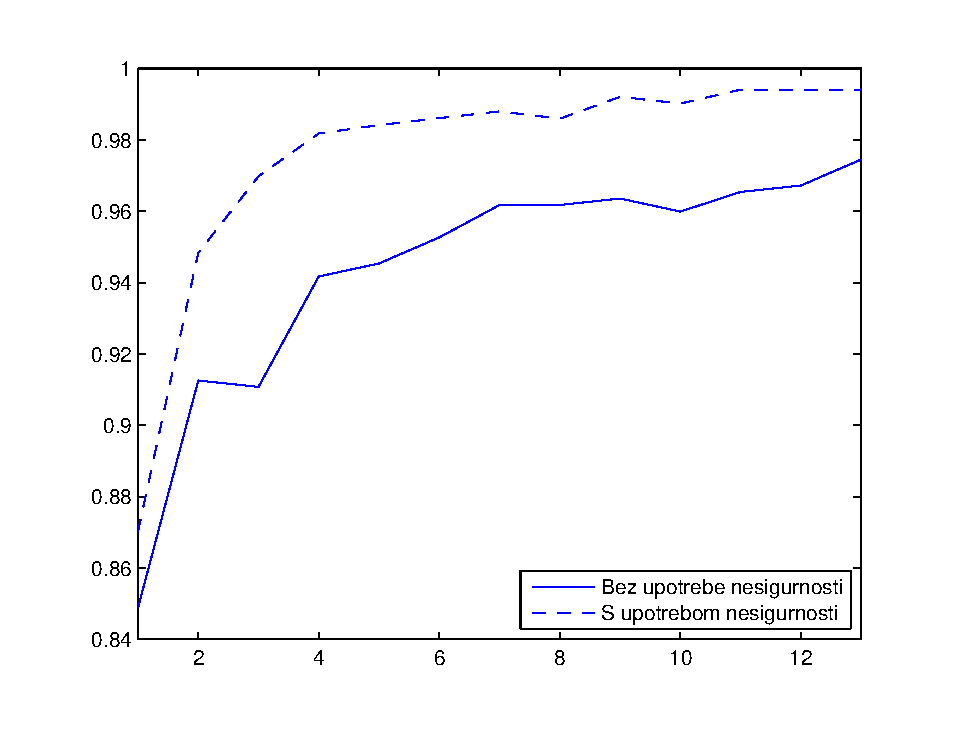
\includegraphics[scale=0.5]{accByClassifCount.eps}
	\label{figure:rezPoBrojuKlas}
	\end{figure}
}

\subsection[Po broju dimenzija]{Po broju dimenzija}
\frame{
	\frametitle{Rezultati po broju korištenih dimenzija}
	\begin{columns}[htb]
		\column{.5\textwidth}
			\begin{figure}
			\centering
			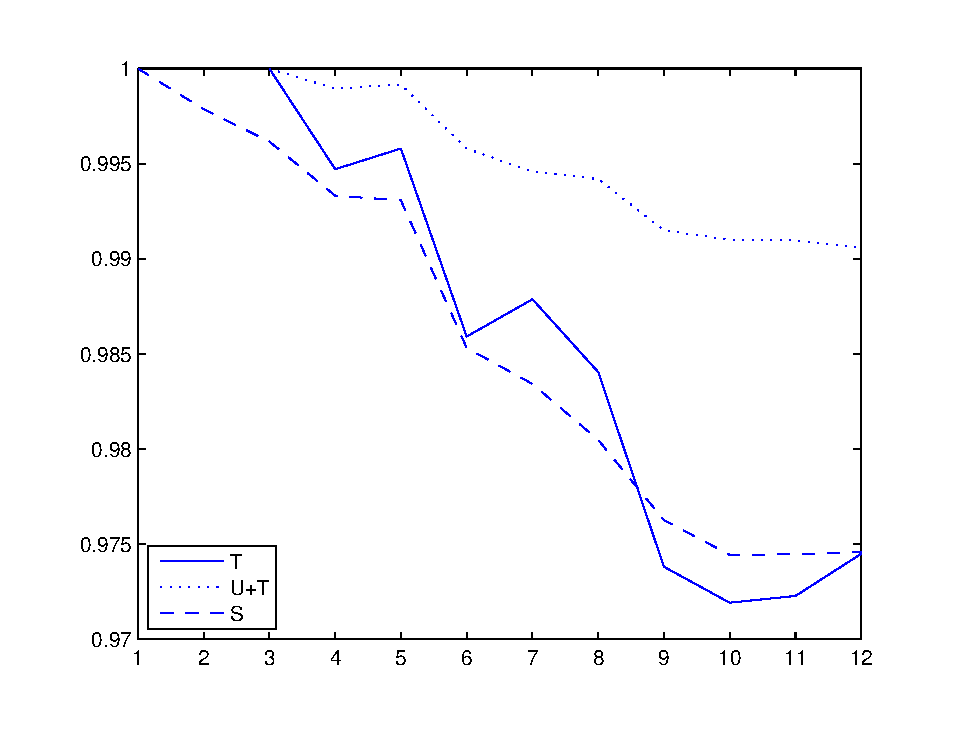
\includegraphics[scale=0.34]{accByDim1.eps}
			\caption{Bez upotrebe nesigurnosti}
			\end{figure}
		\column{.5\textwidth}
			\begin{figure}
			\centering
			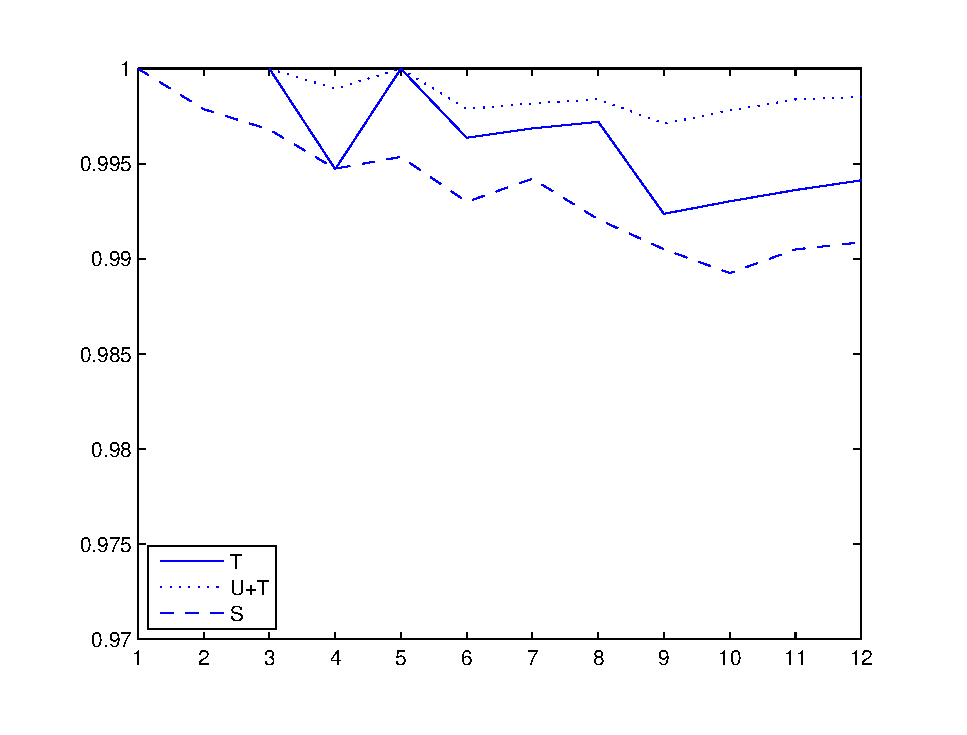
\includegraphics[scale=0.34]{accByDim2.eps}
			\caption{Uz upotrebu nesigurnosti}
			\end{figure}
	\end{columns}
	\begin{itemize}
	  \item Primjer: točnost za slova A-F je 99,72\% uz 4,78\% nesigurnih
	\end{itemize}
}

\section[Zaključak]{Zaključak}

\frame{
  \frametitle{Zaključak}
  \begin{itemize}
    \item TODO
  \end{itemize}
}

\frame{
  \frametitle{Literatura}
  
  \beamertemplatebookbibitems
  
  \begin{thebibliography}{10}
    
  \bibitem{knuth:texbook}
    Donald~E.~Knuth
    \newblock {\em The \TeX book}
    \newblock Addison-Wesley, Reading, Massachusetts, 1994.

  \beamertemplatearticlebibitems
  \bibitem{harisimic:latexsistem}
    V.~Hari i D.~Šimić
    \newblock {\em \LaTeX: Sistem za pripremu dokumenata}
    \newblock \texttt{http://www.math.hr/\textasciitilde hari/skr.dvi}
  \end{thebibliography}
}

\end{document}